%%%%%%%%%%%%%%%%%%%%%%%%%%%%%%%%%%%%%%%%%
% University/School Laboratory Report
% LaTeX Template
% Version 3.1 (25/3/14)
%
% This template has been downloaded from:
% http://www.LaTeXTemplates.com
%
% Original author:
% Linux and Unix Users Group at Virginia Tech Wiki 
% (https://vtluug.org/wiki/Example_LaTeX_chem_lab_report)
%
% License:
% CC BY-NC-SA 3.0 (http://creativecommons.org/licenses/by-nc-sa/3.0/)
%
%%%%%%%%%%%%%%%%%%%%%%%%%%%%%%%%%%%%%%%%%

%----------------------------------------------------------------------------------------
%	PACKAGES AND DOCUMENT CONFIGURATIONS
%----------------------------------------------------------------------------------------

\documentclass[UTF8]{ctexart}

\usepackage{siunitx} % Provides the \SI{}{} and \si{} command for typesetting SI units
\usepackage{graphicx} % Required for the inclusion of images
\usepackage{graphics}%图片设置
\usepackage{subfigure} 

\usepackage{natbib} % Required to change bibliography style to APA
\usepackage{amsmath} % Required for some math elements 
\usepackage{amssymb} % 使用因为所以符号
\usepackage{fancyhdr} % 使用页眉

\usepackage{algorithm}
\usepackage{algorithmic}

\usepackage{listings} % 插入代码
\usepackage{xcolor}
\lstset{
    %backgroundcolor=\color{red!50!green!50!blue!50},%代码块背景色为浅灰色
    rulesepcolor= \color{gray}, %代码块边框颜色
    breaklines=true,  %代码过长则换行
    numbers=left, %行号在左侧显示
    numberstyle= \small,%行号字体
    %keywordstyle= \color{red},%关键字颜色
    commentstyle=\color{gray}, %注释颜色
    frame=shadowbox%用方框框住代码块
    }

%\usepackage{url} % 引用URL
% \usepackage{cite}
% \newcommand{\upcite}[1]{\textsuperscript{\textsuperscript{\cite{#1}}}} %参考文献上标
%\bibliographystyle{plain}   %引用的样式%

\pagestyle{fancy}
\fancyhf{} 
\cfoot{\thepage} 

\setlength\parindent{0pt} % Removes all indentation from paragraphs

\renewcommand{\labelenumi}{\alph{enumi}.} 

%----------------------------------------------------------------------------------------
%	DOCUMENT INFORMATION
%----------------------------------------------------------------------------------------
\title{算法分析与设计-作业四}

\author{王宸昊 2019214541}

\date{\today}

\begin{document}

\maketitle

%----------------------------------------------------------------------------------------
%	SECTION 1
%----------------------------------------------------------------------------------------

\section{CLRS, Page, 210 15.1-4}

\subsection{实现思路}

使用s[i]来记录切割点的坐标,在每次更新状态值时,记录相应的位置信息。\\
递归结束后,依次寻找切分点。\\

\subsection{实现代码}

\begin{lstlisting}[language={python}]
    # 动态规划-带备忘录的自顶向下方法-记录路径
    def Extended_Memoized_Cut_Rod(p, n):
        r = [-1] * (n + 1)
        s = [0] * (n + 1)  # 记录最优解路径
        Extended_Memoized_Cut_Rod_Aux(p, n, r, s)
        print(r)
        print(s)
        print("最优解:%d" % r[n])
        print("最优路线:")
        while n > 0:
            print(s[n])
            n = n - s[n]

    def Extended_Memoized_Cut_Rod_Aux(p, n, r, s):
        if r[n] >= 0:
            return (r[n])
        if n == 0:
            max_value = 0
        else:
            max_value = -1
        for i in range(1, n+1):
            temp = Extended_Memoized_Cut_Rod_Aux(p, n-i, r, s)
            if max_value < p[i] + temp:
                max_value = p[i] + temp
                s[n] = i    # 记录最优时切分点的位置
        r[n] = max_value    # 记录下n时的最小值
        
        return max_value
\end{lstlisting}

\subsection{输出结果}

\begin{figure}[H]
    \centering
    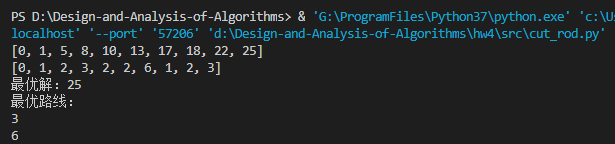
\includegraphics[width=1\textwidth]{img/res-1.png}
    \caption{不同规模下排序算法时间对比}
    \label{带切割方案的备忘录方法}
\end{figure}


%----------------------------------------------------------------------------------------
%	SECTION 2
%----------------------------------------------------------------------------------------

\section{CLRS, Page, 222 15.3-4}

证明:\\
假设现在有四个矩阵:$A_1, A_2, A_3, A_4$,输入的维度序列$ p = [1000, 100, 20, 10,1000] $。\\
Capulet教授的算法为贪心策略,每次选择使$p_0 * p_k * p_4$最小的k值。所以第一次选择k=3时,将矩阵乘法顺序变为$((A_1A_2A_3)A_4)$,第二步选择k=2,将顺序调整为$(((A_1A_2)A_3)A_4)$。总的乘法计算次数为$1000*100*20 + 1000*20*10 + 1000 * 10 * 1000 = 12,200,000$。\\

而当计算顺序为:$((A_1(A_2A_3))A_4)$时,总的乘法计算次数为$100*20*10 + 1000*100*10 + 1000 * 10 * 1000 = 11,020,000$。\\

由此可见,只采用贪心的策略可能会得到次优解。
  
%----------------------------------------------------------------------------------------
%	SECTION 3
%----------------------------------------------------------------------------------------

\section{基于接缝裁剪的图像压缩}

\subsection{证明}
假设在第i行的接缝数量为$S_i$,由算法原理可知,在第i-1行中的接缝位置一定在其上方或者左上或者右上,除了左右边界以外,对每行的接缝都有3种可能。因此此时的接缝可能数为$3^m$。假如在每行中都是边界,则接缝的可能数是$2^m$。综上,接缝的数量是m的指数函数。

\subsection{算法原理}

算法的主要执行过程如下:
\begin{enumerate}
    \item 对输入的图像每个像素计算一个能量图
    \item 对于二维的能量图,找到一条能量值最小的八联通路径
    \item 删除能量最小的路径
    \item 重复以上步骤,满足缩放的比例
\end{enumerate}

\textbf{能量图}:在算法的第一步,需要对每个像素计算能量图。能量图代表了每个像素点所代表的能量的大小,可以直观的理解为像素的变化程度,例如天空、水面等变化比较小的场景所具有的能量就比较小。\\
在具体计算的时候,我采用的方法是使用sobel滤波器,对图像的RGB三个通道进行卷积,然后将其绝对值加起来,变成能量图。采用的sobel算子如下:
\begin{equation*}
    d_u = 
    \begin{bmatrix}
        +1 & +2 & +1 \\
        0 & 0 & 0 \\
        -1 & -2 & -1
    \end{bmatrix} 
    d_v = 
    \begin{bmatrix}
        +1 & 0 & -1 \\
        +2 & 0 & -2 \\
        +1 & 0 & -1
    \end{bmatrix}     
\end{equation*}

\textbf{能量图}:寻找能量最小的路径,是一个动态规划问题,从图像的上边缘开始,自顶向下寻找一条路径。$dp[i][j]$到当前点的最小能量值,$energy\_map[i][j]$表示当前点的能量值,则dp的关系如下:
\begin{equation*}
    dp[i][j] = energy\_map[i][j] + min(dp[i-1][j-1], dp[i-1][j], dp[i-1][j+1])
\end{equation*}

\textbf{删除能量最小的路径}:用一个辅助数组backtrack[i][j]记录上一层的j坐标,依次回溯,即可找到最小能量路径,将其删除即可。\\

综合以上分析,针对一副$m*n$的图片,删除一条像素线的算法复杂度为$O(mn)$

\subsection{伪代码}

\begin{lstlisting}
CALC_ENERGY(img)
    let filter_du[3][3], filter_dv[3][3] be sobel filter
    convolved = |convolve(img, filter_du)| + |convolve(img, filter_dv)|
    energy_map = convolved.sum()

    return energy_map

MIN_SEA(img)
    let dp[0..m][0..n],backtrack[0..m][0..n] be new arrays
    dp[1..m][0]=0
    dp[0][1..n]=0
    for i=1 to m
        for j=1 to n
            dp[i][j] = energy_map[i][j] + min(dp[i-1][j-1], dp[i-1][j], dp[i-1][j+1])
            backtrack[i][j] = min_j
    
    return dp,backtrack
\end{lstlisting}

\subsection{算法效果}
cd到src目录下,使用 $seam\_carving.py -i <inputfile> -o <outputfile> -r <row_rate> -c <column_rate> $运行脚本。\\

第一张实验图是一张800*533的风景图,row\_rate设置为0.5, column\_rate设置为0.4,压缩后照片大小为320*266,处理前后效果如下:

\begin{figure}[H]
    \centering
    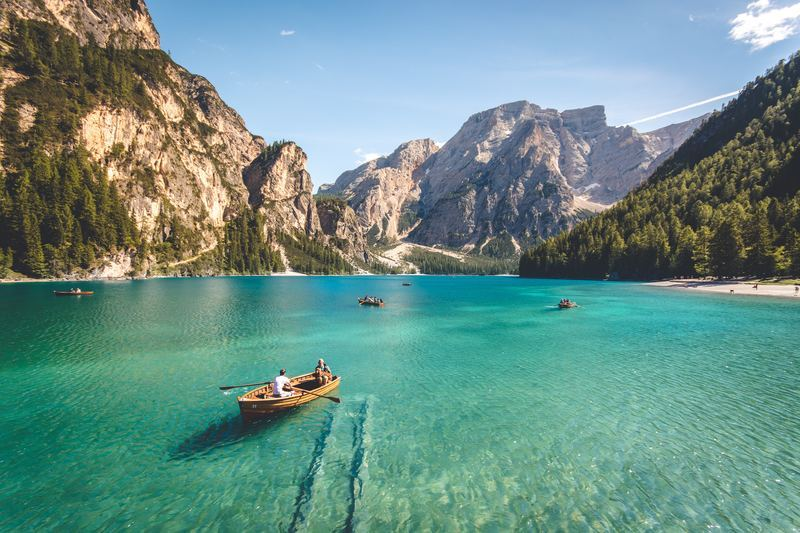
\includegraphics[width=1\textwidth]{img/input-1.jpg}
    \caption{风景图处理前}
    \label{input-1}
\end{figure}

\begin{figure}[H]
    \centering
    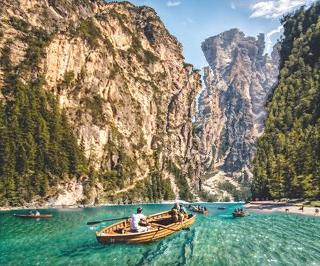
\includegraphics[width=1\textwidth]{img/output-1.jpg}
    \caption{风景图处理后}
    \label{output-1}
\end{figure}
从效果看,经过压缩好很好的保留了水面上的主体船,裁剪的部分主要是水面和天空,像素比较接近的地方。

第二张实验图是一张537*401的苹果在桌子上的图,row\_rate设置为0.8, column\_rate设置为0.8,压缩后照片大小为429*320,处理前后效果如下:
\begin{figure}[H]
    \centering
    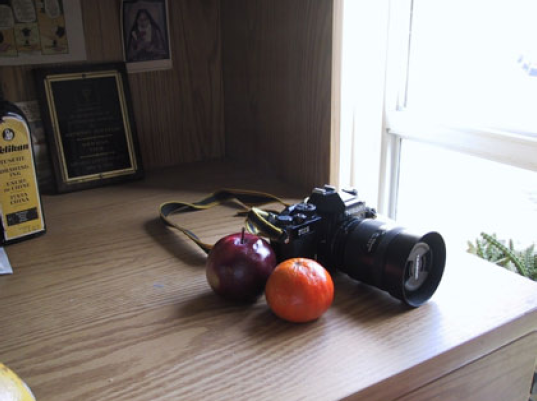
\includegraphics[width=1\textwidth]{img/input-2.png}
    \caption{相机图处理前}
    \label{input-2}
\end{figure}

\begin{figure}[H]
    \centering
    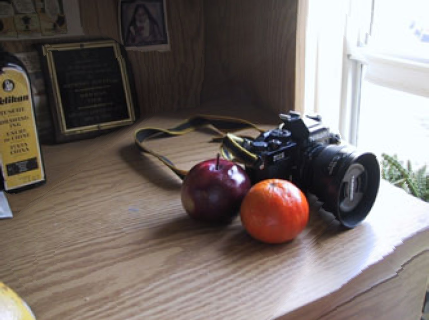
\includegraphics[width=1\textwidth]{img/output-2.png}
    \caption{相机图处理后}
    \label{output-2}
\end{figure}

这张图片的构图比较复杂,主体不仅仅只有一个,从效果看上,比较好的保留了后面的酒瓶和水果和相机,但是相机的镜头稍微有一些变形,这是因为镜头的像素比较接近,能量值比较小,被裁剪掉了一些像素,导致了有稍微的变形。最后,可以明显的观察到桌角的部分有变形的现象。\\

第三张实验图是一张1280*854的人像图,row\_rate设置为0.8, column\_rate设置为0.8,压缩后照片大小为1024*683(由于计算比较耗时,这里保留的rate比较高),处理前后效果如下:
\begin{figure}[H]
    \centering
    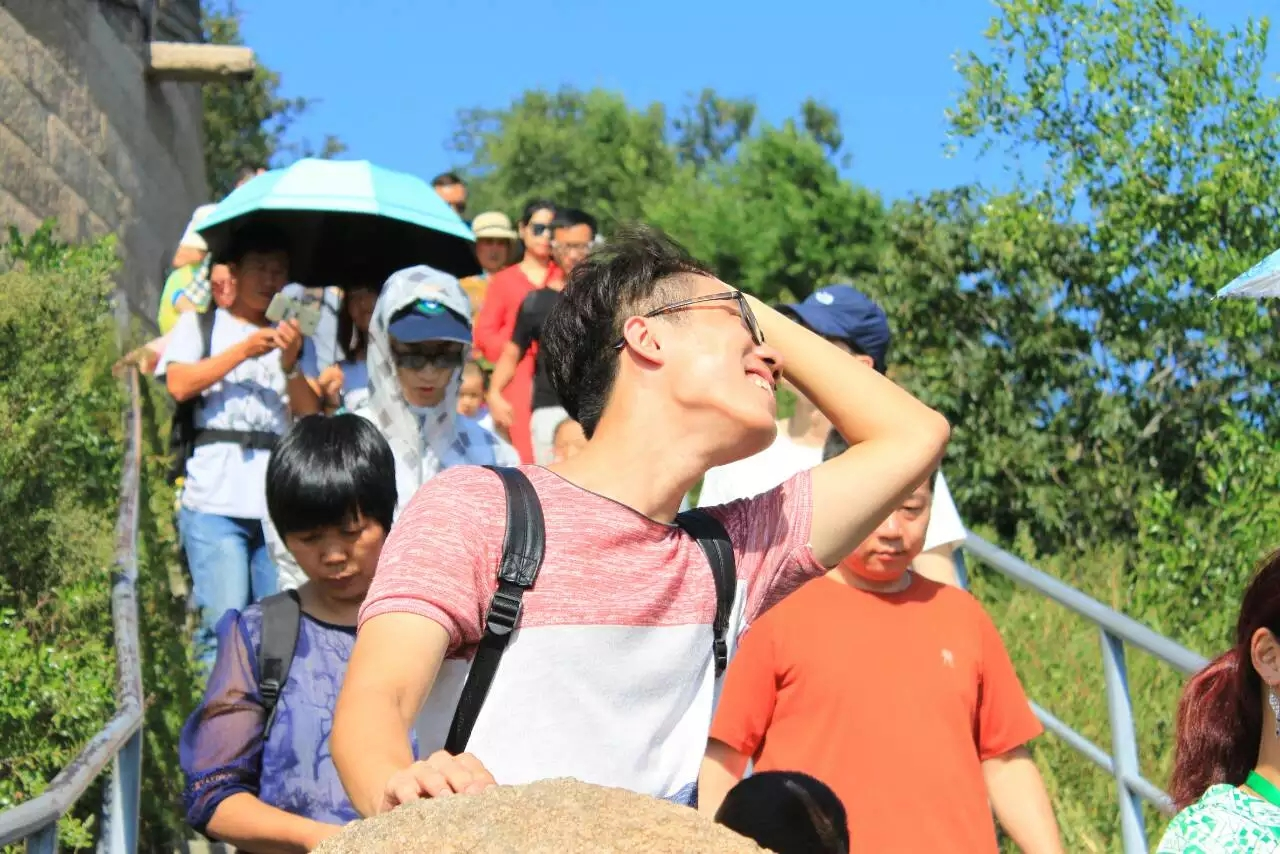
\includegraphics[width=1\textwidth]{img/input-3.jpg}
    \caption{人像处理前}
    \label{input-3}
\end{figure}

\begin{figure}[H]
    \centering
    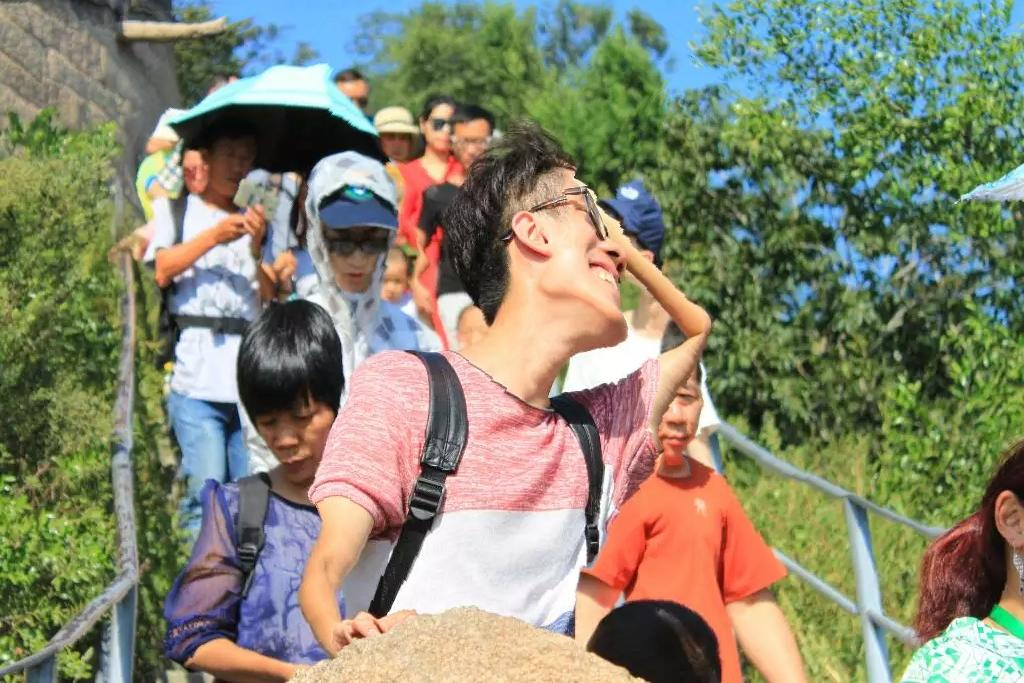
\includegraphics[width=1\textwidth]{img/output-3.jpg}
    \caption{人像处理后}
    \label{output-3}
\end{figure}
可以看出在整体色彩都比较鲜艳,主体不太明显的情况下,使用该算法的效果并不好。由于各个像素点的变化比较明显,所以算出的能量值差异并不明显,由此进行裁剪时,对造成图片的变形。\\

综合以上可以得出,seam\_carving算法比较适合风景图,或者是主体的特征比较明显的,这是因为主体的能量明显高于周围背景,不容易被裁剪掉,从而在压缩中可以更好地保留下来主体。


\end{document}